\begin{figure} 
  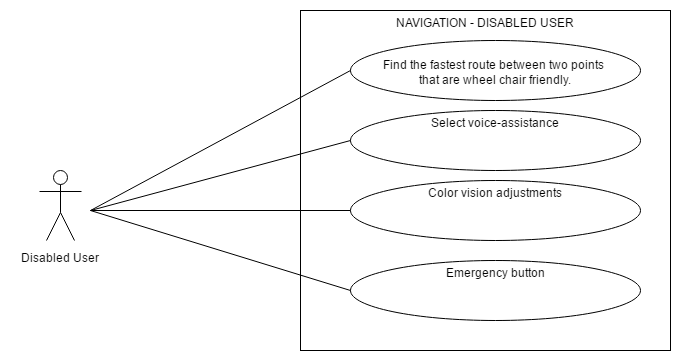
\includegraphics[width=\textwidth]{diagrams/Specific_Requirements/Disabled_User_Use_Case_Diagram.png}
\end{figure}

The Disabled User Requirements extends from the Logged in or Guest User Requirements. The aim of the disabled navigation is to accommodate disabled users be it students, employees or visitors to successfully use the system.
\\
\bigskip

\FuncReq
{Select voice-assistance.}
{The user can select the voice assistance function so that the mobile application may use voice-commands instead of manually selecting the mobile application's functions.}
{Trivial}
{Voice assist is enabled}
    \\
    \textbf{Actor system interaction model: Select voice-assistance.}\\
    \begin{tabular}{ | p{6cm} | p{6cm} |}
    \hline
    Actor: Disabled User & System: NavUp \\ \hline
     & 0. The mobile app displays an option to choose a voice command function to communicate with the user.\\ \hline
    1. The user selects to employ the functionality. & 2. The application communicates to the user by use of audible commands as well as a visual representation.\\ \hline
    3. The user may respond in the form of a voice command or by using the touch interface on the mobile device. & \\ \hline
    
    \end{tabular}
\\
\bigskip

\FuncReq
{Color blind}
{The user is able to adjust the color displayed on the mobile device to accommodate various kinds of colour blindness.}
{Trivial}
{Mobile app has changed its colour scheme to accommodate the selected type of colour blindness}
    \\
    \textbf{Actor system interaction model: Color blind}\\
    \begin{tabular}{ | p{6cm} | p{6cm} |}
    \hline
    Actor: Disabled User & System: NavUp \\ \hline
     & 0. The mobile app displays a menu to choose a colour scheme that accommodates the user.\\ \hline
    1. The user selects their type of colour blindness. & 2. The mobile app adjusts the colour scheme to accommodate the type of colour blindness.\\ \hline   
    \end{tabular}
\\
\bigskip

\FuncReq
{View the map of campus.}
{This feature extends on the base user functionality for viewing a map but also accommodates the selected disability. This can be in the form of changing the colour scheme for the colour blind or ramp locations for the physically disabled. It should also indicate the location of the disability unit on campus.}
{User cannot be blind}
{Mobile app has adjusted its output to suite the selected disability}

\FuncReq
{Search for a location/venue on campus to be displayed on the map}
{This feature extends on the base user functionality for searching for a location. The mobile app should allow searching of locations by voice command}
{Disablility only applies to disabilities that require voice command}
{Trivial}

\FuncReq
{Find the fastest route between two points that are wheel chair friendly.}%This functional requirement will include finding the start point by gps or by manual input from the user
{This feature extends on the base user functionality for fastes route finding. The mobile application will navigate a path for the user that is disabled and wheelchair friendly, allowing them to navigate with minimal obstruction.}
{The user has indicated his/her disability in the accessibility options}
{Trivial}

\FuncReq
{View various points of interest.}
{This feature extends on the base user functionality of viewing various points of interest but includes the functionality to accommodate certain disabilities. In the case of the blind, the mobile app will ask the user if he/she would like to hear about the points of interest.}
{Trivial}
{Trivial}

\FuncReq
{View any current events or activities happening on campus.}
{This feature extends on the base user functionality for viewing current events and activities but includes the functionality to accommodate certain disabilities.In the case of the blind, the mobile app will ask the user if he/she would like to hear about any current events or activities happening on campus.}
{Trivial}
{Trivial}

\FuncReq
{Emergency button.}
{The user can use this special feature to alert the system in the event of an emergency so that nearest wheel chair friendly route to exit point for the disabled user can be displayed.The feature uses the current location of the user to find the fastest wheel chair friendly route.}
{Trivial}
{Emergency personnel are sent to assist the user.}
    \\
    \textbf{Actor system interaction model: Emergency Button}\\
    \begin{tabular}{ | p{6cm} | p{6cm} |}
    \hline
    Actor: Disabled User & System: NavUp \\ \hline
      & 0. The mobile application will display an emergency button or respond to a push event from the remote repository.\\ \hline
      & 1. The emergency personnel are notified and are provided with the location of the user.\\ \hline   
    \end{tabular}
\\
\bigskip
